\section{Parring i grafer}
Nogle grafer har den egenskab, at deres knuder kan deles op i to undergrupper, således at knuder fra dan samme undergruppe ikke forbindes af kanter, men kun forbindes med knuder fra den anden undergruppe.
Dette kaldes parring i grafer.
Parring i grafer kan blandt andet bruges til at vise relationer mellem to forskellige typer objekter.
Et eksempel på dette kan være en graf, der viser hvilke studerende der tager hvilke kurser, så de studerende er i en undergruppe og kurserne i en anden. 

\begin{defn}
En simpel graf $G$ kaldes parret, hvis dens knuder kan deles op i to adskilte undergrupper $V_1$ og $V_2$, så hver kant i grafen forbinder en knude fra $v_1$ og $V_2$, men ikke to knuder fra den samme undergruppe.
Når dette gælder, kaldes parret ($V_1,V_2$) en parring af $V$ i $G$.
\end{defn}

\begin{exmp}
I Figur \ref{parret_graf} ses en parret graf, med de to undergrupper ($v1,v2,v3$) og ($v3,v4$). 
På grafen ses det, at hvert kant forbinder en knude fra den ene undergruppe med en fra den anden, mens ingen kanter forbinder to knuder fra den samme undergruppe. 
Deruder ses det også, at der ikke er en kant fra alle knuder i en gruppe til alle knuder i den anden undergruppe.
Der er for eksempel ikke en kant mellem $v3$ og $v5$. 
Der behøver ikke være kanter fra alle knuder i den ene undergruppe til den anden for at grafen er parret.
Havde der været en kant mellem $v1$ og $v2$ havde grafen ikke været parret, da der ikke må være en kant mellem to knuder fra samme undergruppe.
\end{exmp}

\begin{figure}[h]
\centering
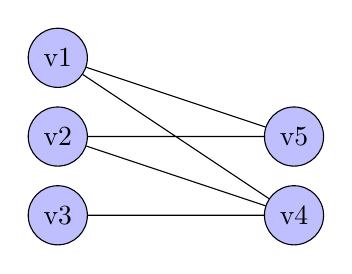
\begin{tikzpicture}[every node/.style={draw,shape=circle,fill=blue!25}]
\path (-1.5,0) node (p0) {v1}
(-1.5,-1) node (p1) {v2}
(-1.5,-2) node (p2) {v3}
(1.5,-2) node (p3) {v4}
(1.5,-1) node (p4) {v5};
\draw 
(p0) -- (p3) 
(p0) -- (p4)
(p1) -- (p3)
(p1) -- (p4)
(p2) -- (p3);
\end{tikzpicture}
\caption{Parret graf}
\label{parret_graf}
\end{figure}

\begin{thm}
En simpel graf er parret hvis og kun hvis, det er mulig at tildele hver knude en af to farver, således at hver kant ikke forbinder to knuder af samme farve. 
\label{farve_satning}
\end{thm}

\begin{proof}
Antag at $G=(V,E)$ er en parret simpel graf. Så er $V=V_1 \cup V_2$, hvor $V_1 \cap V_2 = Ø$ og hver kant i E forbinder en knude i $V_1$ med en knude i $V_2$. 
Tildeles en farve til alle knuder i $V_1$ og en anden farve til alle knuderne i $V_2$, så vil ingen kanter forbinde to knuder af samme farve. 
Gå så ud fra, at det er muligt at tildele farver til knuder, hvor der kun bruges to farver, hvor hvert knudepar består af to knuder af hver sin farve.
Når det gælder er $V_1 \cap V_2=Ø$ og $V=V_1 \cup V_2$.
Ydermere forbinder hver kant en knude i $V_1$ til en knude i $V_2$, da ingen naboknuder kan tilhøre samme undergruppe. 
\end{proof}

\begin{exmp}
I Figur \ref{farve_graf} ses en parret graf, hvor hver knude er tildelt en farve jævnfør sætning \ref{farve_satning}. 
Her ses det, hvordan hevr kant forbinder en rød knude med en blå knude, samt hvordan ingen kant forbinder to røde eller to blå knuder.

\begin{figure}[h]
\centering
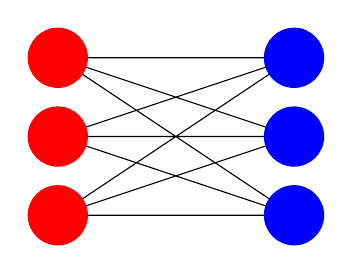
\begin{tikzpicture}[every node/.style={draw,shape=circle,fill=blue!25}]
\path (-1.5,0) node (p0) [red]{v1}
(-1.5,-1) node (p1) [red]{v2}
(-1.5,-2) node (p2) [red]{v3}
(1.5,-2) node (p3) [blue]{v4}
(1.5,-1) node (p4) [blue]{v5}
(1.5,0) node (p5) [blue]{v6};
\draw 
(p0) -- (p3)
(p0) -- (p4)
(p1) -- (p3)
(p1) -- (p4)
(p2) -- (p3)
(p2) -- (p4)
(p5) -- (p0)
(p5) -- (p1)
(p5) -- (p2);
\end{tikzpicture}
\caption{Farveopdelt parret graf}
\label{farve_graf}
\end{figure}
\end{exmp}

En parret graf kan siges at være komplet. 
At en graf er komplet betyder, at hver knude fra en undergruppe er forbundet med alle knuder fra den anden undergruppe. 
En sådan graf betegnes $K_m,n$, hvor m er antallet af knuder i den ene undergruppe og n antallet i den anden undergruppe. 

\begin{exmp}
Grafen i Figur \ref{farve_graf} er også en komplet parret graf, fordi hver rød knude er forbundet med hver blå knude. 
Denne graf kaldes derfor $K_{3,3}$
\end{exmp}
